\chapter{An Overview of Snapstore}

Snapstore was created with two distinct groups of users in mind, non-technical users and technical users. In order to be an attractive system to technical users who use systems like Git, Snapstore needed to support the functionality of powerful version control systems. However, Snapstore also needed to have a smoother learning curve to promote quick startup and attract users who feel overwhelmed by complicated VCSs. 

Snapstore's vision is that of an opt-in strategy concerning complexity. Users can download Snapstore and get started right away with simple actions like file backup. Then, if desired, users can explore more advanced features of the system.

Snapstore operates within a specially designated Snapstore folder which is created upon opening the application for the first time. It is similar to the Dropbox folder; Snapstore only looks at files that are inside of it. Snapstore watches the user's filesystem for changes in order to respond with certain actions like creating snapshots (section 2.1.1). This allows users to use any editor with Snapstore.

\section{Basic Concepts}

The basic features of Snapstore allow a single user to use the application like they would a file syncing system.

\subsection{Snapshots}

\textit{Snapshots} allow a user to persistently store all of their edits to a file over time. Whenever a file is saved to disk, a snapshot is created with the contents of that file and stored in the local repository. Snapshots can be the result of a create, update, rename, delete, merge, or conflicting merge of a file. Users can retrieve an old state of a file by finding the appropriate snapshot in the file's history.

Snapshots are created when a file is created, updated, deleted or renamed. Snapshots are also created when files are merged together. These snapshots are either the result of a successful merge or of a conflicting merge. Snapshots, then, can be one of six types: create, update, delete, rename, merge, or conflict.

When creating snapshots for a given file, Snapstore will add the snapshot to that file's \textit{snapshot graph}. This graph represents the history of the file and it shows each snapshot that was taken, along with its relationship to other snapshots of that file. A snapshot has one or more parents (the snapshot(s) taken before it), and it has a child (the snapshot taken after it). A Snapshot can have more than one parent if it is a product of a merge of multiple snapshots. The first snapshot in a graph is called the \textit{root}. The last snapshot in the graph is called the \textit{head}. The contents of a file's head snapshot will always match the contents of the file on disk.

Figure 2-1 shows how to navigate a file's snapshot graph in Snapstore. You first find that file within Snapstore's interface. In this example we choose ``foo.txt''. Clicking on the file's name makes the snapshot graph appear at the top of the window. Each node in this graph is a snapshot, and the node on the far right is the head. When you click on these nodes, the content of that snapshot will appear on the bottom-right of the window. In this example we select the second snapshot, 1. To revert to this snapshot, click ``Revert'', a button above the snapshot content. Reverting to a previous snapshot creates the new snapshot, 4, with the same content as snapshot 0 and alters the file's content on disk to match the new head snapshot.

\begin{figure}
\begin{center}
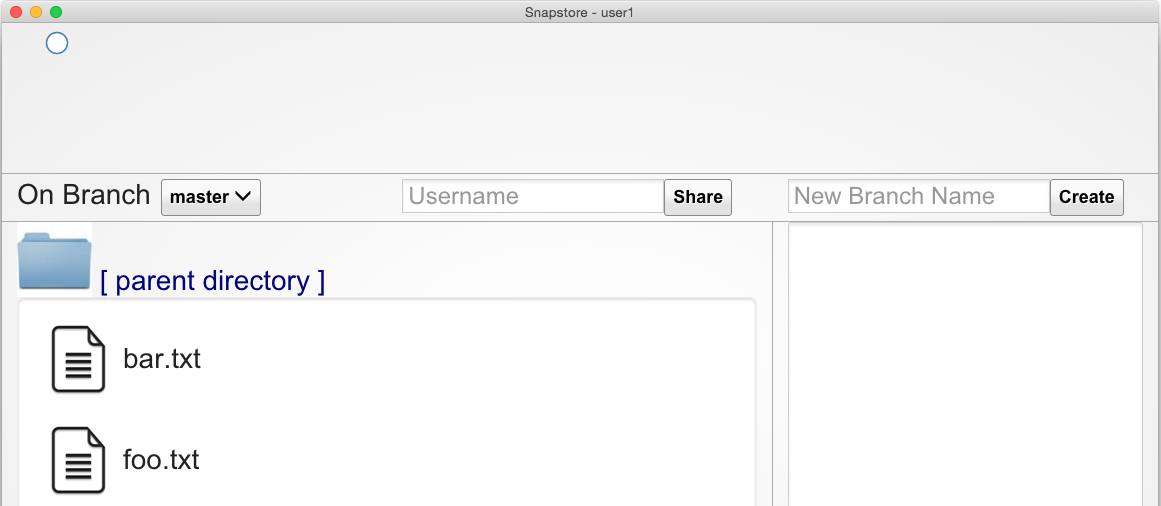
\includegraphics[width=0.72\textwidth]{SnapshotGraph1-crop}
\vspace{3 mm}
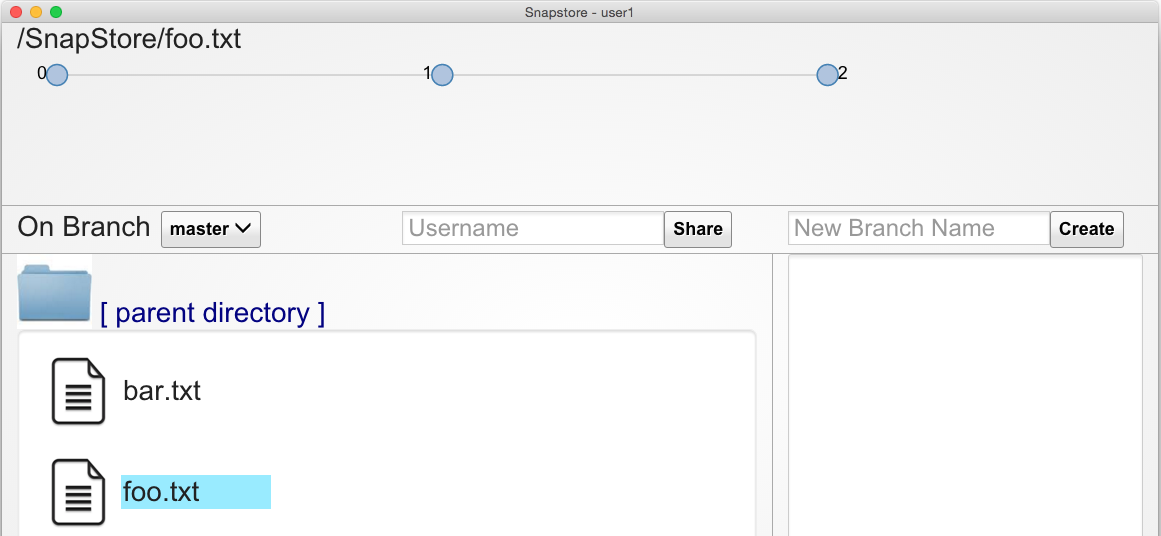
\includegraphics[width=0.72\textwidth]{SnapshotGraph2-crop}
\vspace{3 mm}
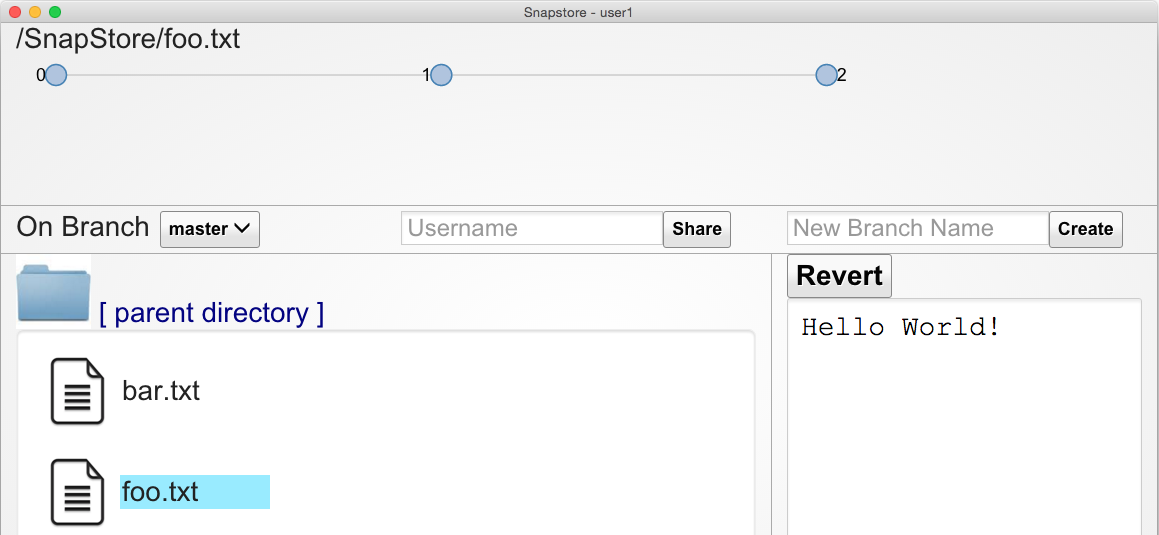
\includegraphics[width=0.72\textwidth]{SnapshotGraph3-crop}
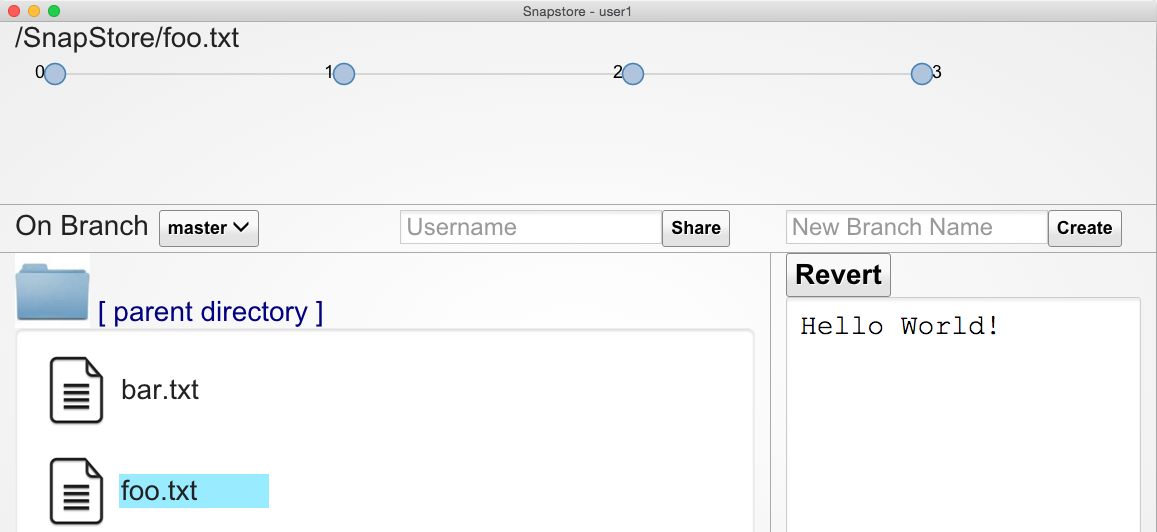
\includegraphics[width=0.72\textwidth]{SnapshotGraph4-crop}
\end{center}
\caption{Locating a file's snapshot graph, choosing a snapshot, and reverting to it.}
\label{arm:fig1}
\end{figure}

\subsection{Upstreams}

\textit{Upstreams} are used to synchronize the data of collaborators on a project. Whenever a user makes any changes to their Snapstore system, those changes are sent to the upstream and out to all other users who are collaborating with that user.

If two users are working together on a project, the upstream will synchronize their snapshots, groups, and tags as they make them. In the case of multiple snapshots coming in to the upstream at the same time, the upstream will resolve the conflict and push the same ordering of snapshots to all users.

Git users can sympathize with the hassle of having to commit, push and then pull data whenever changing computers. Snapstore solves this issue using upstreams. Imagine that a user has a desktop and a laptop computer. Both computers have a file called ``foo.txt'' on them. The user works on their desktop, making edits to ``foo.txt'' in the form of snapshots. When they open Snapstore on their laptop, the upstream pushes all of the snapshots made on the desktop to the laptop. Both computers now have the same version of ``foo.txt''. There is no push/pull model in Snapstore, data is automatically propagated.

By default, the upstream is the Snapstore server, but users might want to change their upstream so their data passes through a known location. To do so, follow these steps:
\begin{enumerate}
  \item{Download the Snapstore server program onto the computer.}
  \item{Run the Snapstore server on that computer.}
  \item{Point the Snapstore client to the desired computer by inputting its IP address into the code.}
\end{enumerate}

\subsection{Local Repository}

The \textit{local repository} allows users to work without an active Internet connection. Whenever a user makes any changes to their Snapstore system, that data is first saved in the local repository, whether there is an Internet connection or not. 

If the local repository is connected to an upstream and there is an Internet connection, Snapstore will copy all of the data in the local repository to the upstream repository. If there is not an Internet connection, Snapstore will wait and push all new changes to the upstream repository when connection is restored.

The local repository does need to be connected to an upstream, however. You can use Snapstore locally, without an Internet connection, with only the local repository.

\section{Advanced Concepts}

Snapstore's advanced features allow users to access the more powerful components of a version control system. They provide additional functionality that users might want when working on projects with complex version control requirements.

\subsection{Groups}

\textit{Groups} allow users to designate a collection of snapshots as related. Users can place any number of snapshots in a group, even if they exist across multiple files. The user can then give this group a name and use this name to find the group later.

A software team collaborating on a project might want to fix a syntax bug in their program. If one user makes a few snapshots in this process, they can then place them in a group and title it ``Fixed syntax bug''. Once created, these snapshots and this group have all been shared with the other team members through the upstream. Team members can easily locate this group and inspect its snapshots to see how the bug was fixed. 

Figure 2-2 shows the process to create a group. Because this functionality is not yet implemented, it is a mock-up of the planned interface. First, click the ``Create Group'' button on the right. The snapshot graphs for each file in this branch (section 2.2.3) will then appear. Choose the snapshots you'd like to include in this group. Then, give the group a name. Finally, click ``Create Group'' to finish. Your group name will now appear in the ``Groups'' dropdown menu.

\begin{figure}
\begin{center}
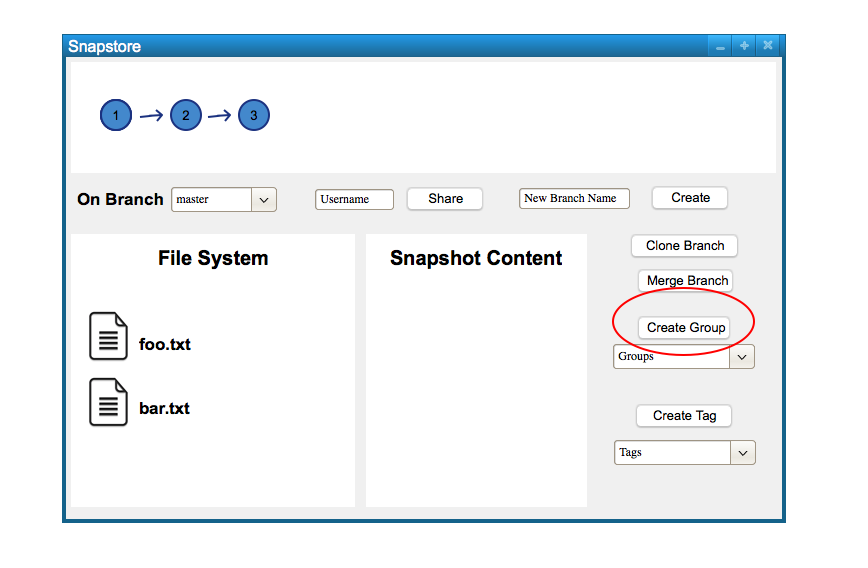
\includegraphics[width=0.72\textwidth]{Group1}
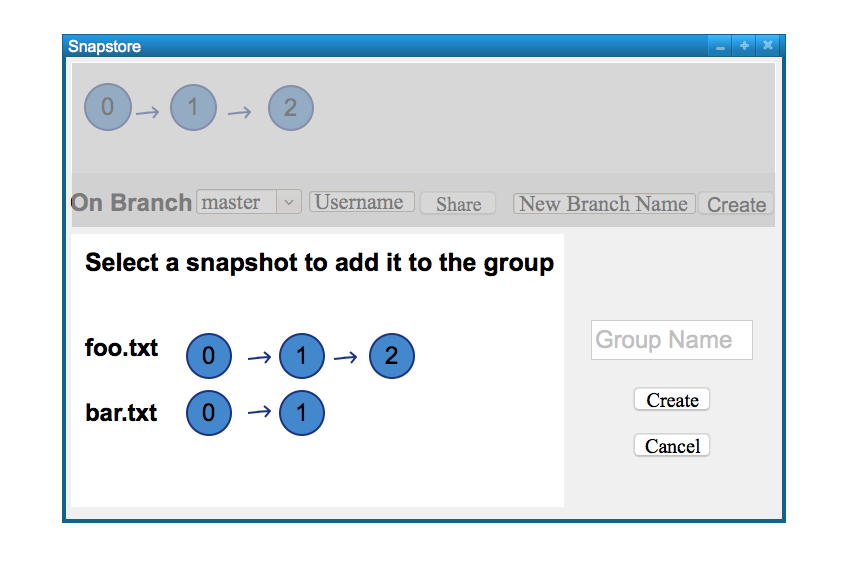
\includegraphics[width=0.72\textwidth]{Group2}
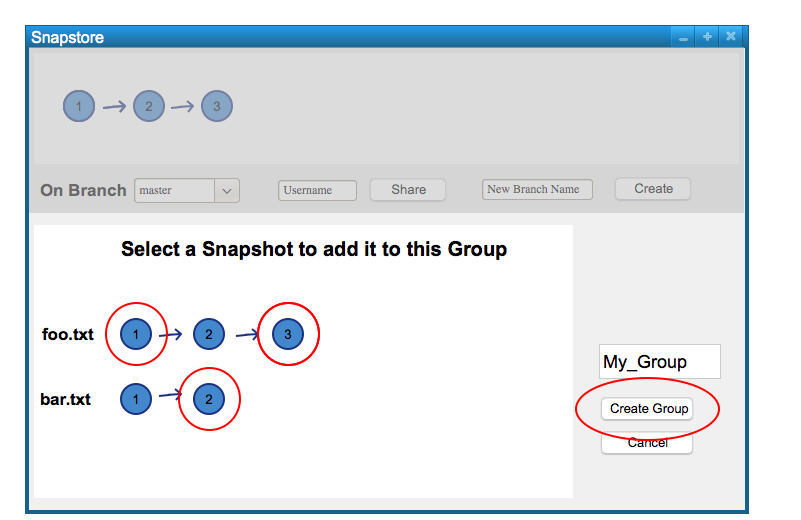
\includegraphics[width=0.72\textwidth]{Group3}
\end{center}
\caption{Creating a Group.}
\label{arm:fig1}
\end{figure}

\subsection{Tags}

\textit{Tags} allow users to designate a group as a coherent point in development. The exact nature of a coherent point will differ from project to project, but in general this means a point in which the project is ready for further development. When a group of snapshots is particularly significant, such as project completion or a release of a piece of software, users can tag that group.

Tags can only be given to groups who have at most one snapshot per file. This is so that the user can revert the state of their files using the tag. When this is done, every file that is in the group with that tag will be reverted to the state described by their snapshot in that group.

One example of using tags is to describe a release in a software project. At the time of the release, a user can tag the group of head snapshots ``Version 1.3'' to signify that the project is in a stable release state. Later, after more snapshots have been created, users can utilize this tag to revert the project to ``Version 1.3''.

\subsection{Branches}

\textit{Branches} allow users to separate independent lines of work. Whenever any data is created, it is saved within the user's current branch. Switching to a different branch will load all data associated with that branch, changing the user's filesystem as necessary. The user can then begin adding data to this branch.

Branches are a collection of snapshots, groups, and tags. The collection of these concepts constitutes an independent line of development. Branches can be shared with other users, making them collaborators on that line of development. Branches can also be merged together in the local repository to combine lines of development.

Snapstore provides a default branch called ``master'' on startup. A user can then create and use new branches to maintain multiple versions/releases of the same project, keep the development of major features isolated, and to give collaborators the ability to try out experimental changes without affecting the main line \cite{RossoJackson}.

Figure 2-3 shows how to create and switch between branches in Snapstore. To create a branch, insert its name into the text box that says ``New Branch Name''. Here we make a new branch called ``development''. Then click create. This will switch you to the new branch, and you can start making snapshots, groups, and tags. To switch back to the ``master'' branch, click the dropdown branch name next to ``On Branch''. This will show you all of your branches. Click the branch you'd like to switch to, in this case ``master'', and you will be placed back on that branch.

\begin{figure}
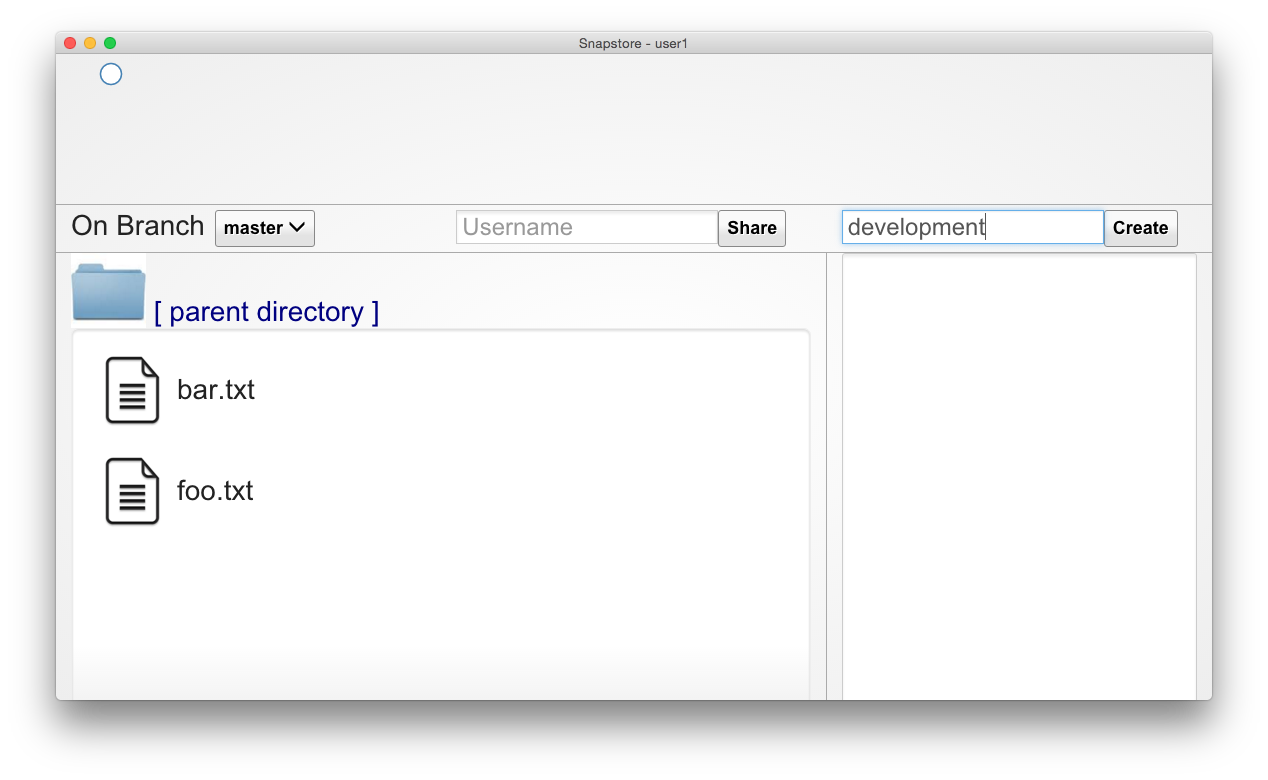
\includegraphics[width=0.5\textwidth]{Branch1}
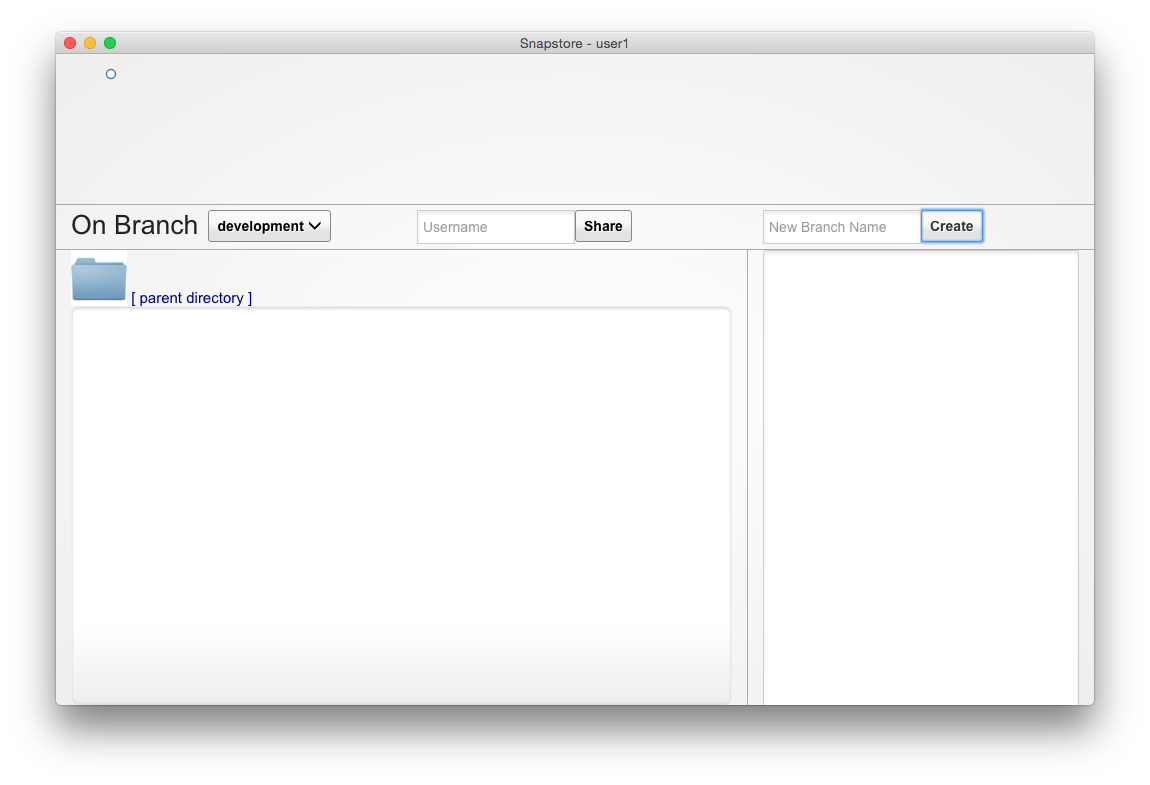
\includegraphics[width=0.5\textwidth]{Branch2}
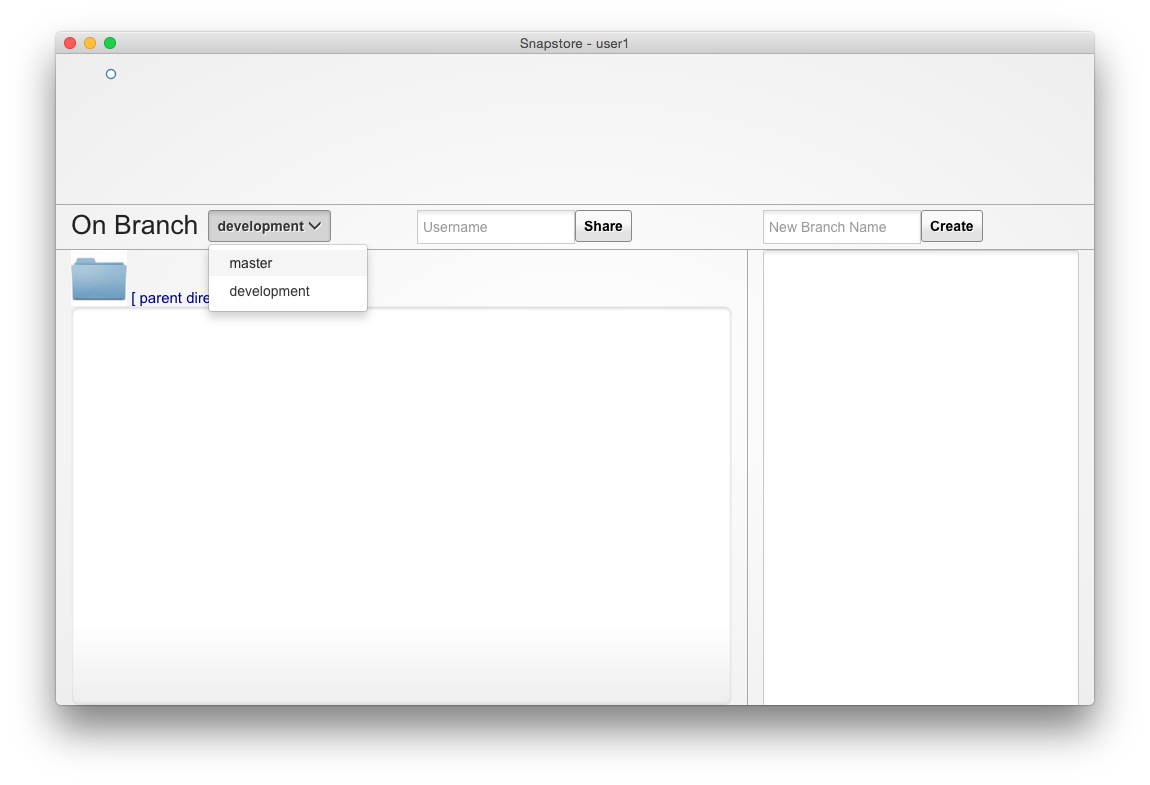
\includegraphics[width=0.5\textwidth]{Branch3}
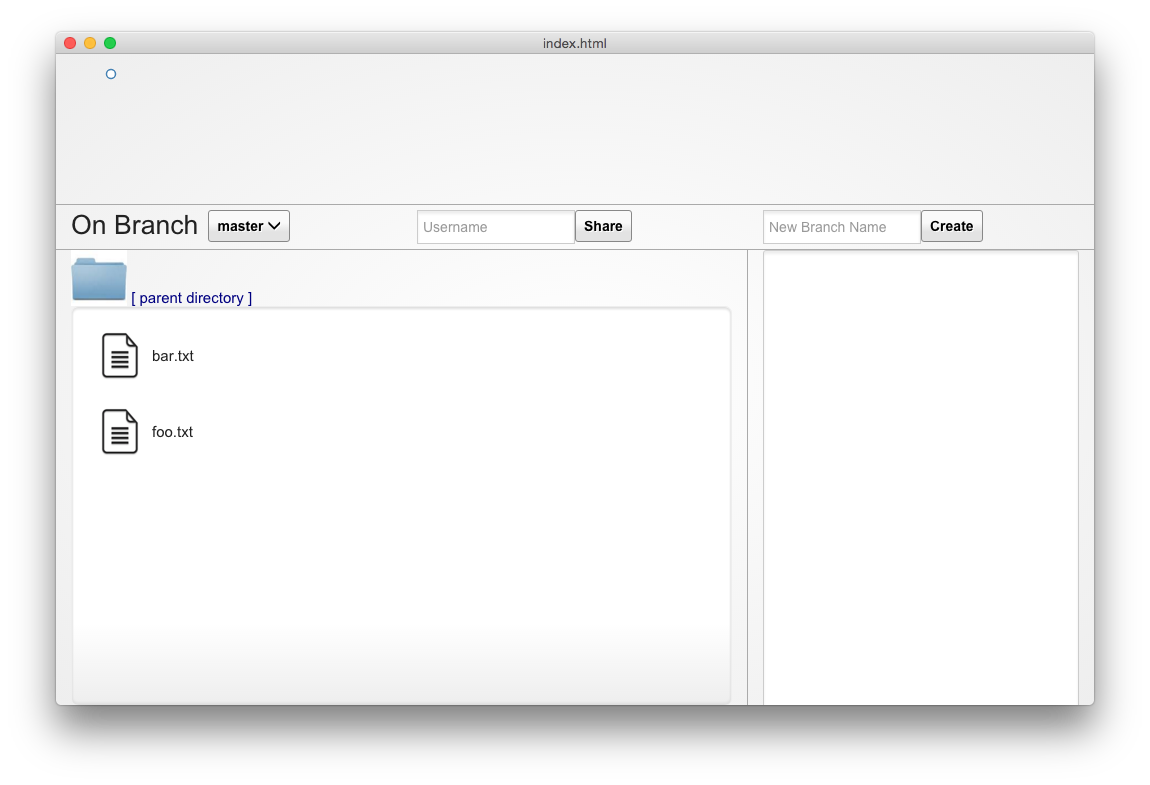
\includegraphics[width=0.5\textwidth]{Branch4}
\caption{Creating a new branch ``development'' and switching back to the ``master'' branch.}
\label{arm:fig1}
\end{figure}

A branch can also be created by cloning an existing branch. Creating a clone involves choosing a branch to clone and selecting snapshots inside the original branch to bring over to the clone. For all snapshots that are cloned into the new branch, any groups associated with those snapshots, and any tags associated with those groups, will be copied to the cloned branch.

\subsubsection{Sharing Branches}

When a branch is shared with another user, that branch's data is copied to that user's local repository. On a shared branch, when any user makes changes, those changes are immediately sent to the other user(s) who are collaborators on that shared branch. For example, one user might create a new snapshot on a file in the shared branch. That new snapshot is propagated to all collaborators on that branch and reflected in their snapshot graphs and on their filesystem.

When conflicts arise due to multiple users working on the same branch at the same time, Snapstore uses a last-write wins rule. The last snapshot to reach the server will become the head snapshot for the file. Other snapshots are placed before the head snapshot in the snapshot graph. No snapshots are lost in the conflict, and the user can revert to a passed over snapshot easily.

Figure 2-4 shows how to share a branch with another user in Snapstore. Navigate to the branch you'd like to share, in this case we're sharing the ``master'' branch. Input the username of the user you'd like to share that branch with in the text box labeled ``Username'' next to the ``Share'' button. Then, click ``Share''.

\begin{figure}
\begin{center}
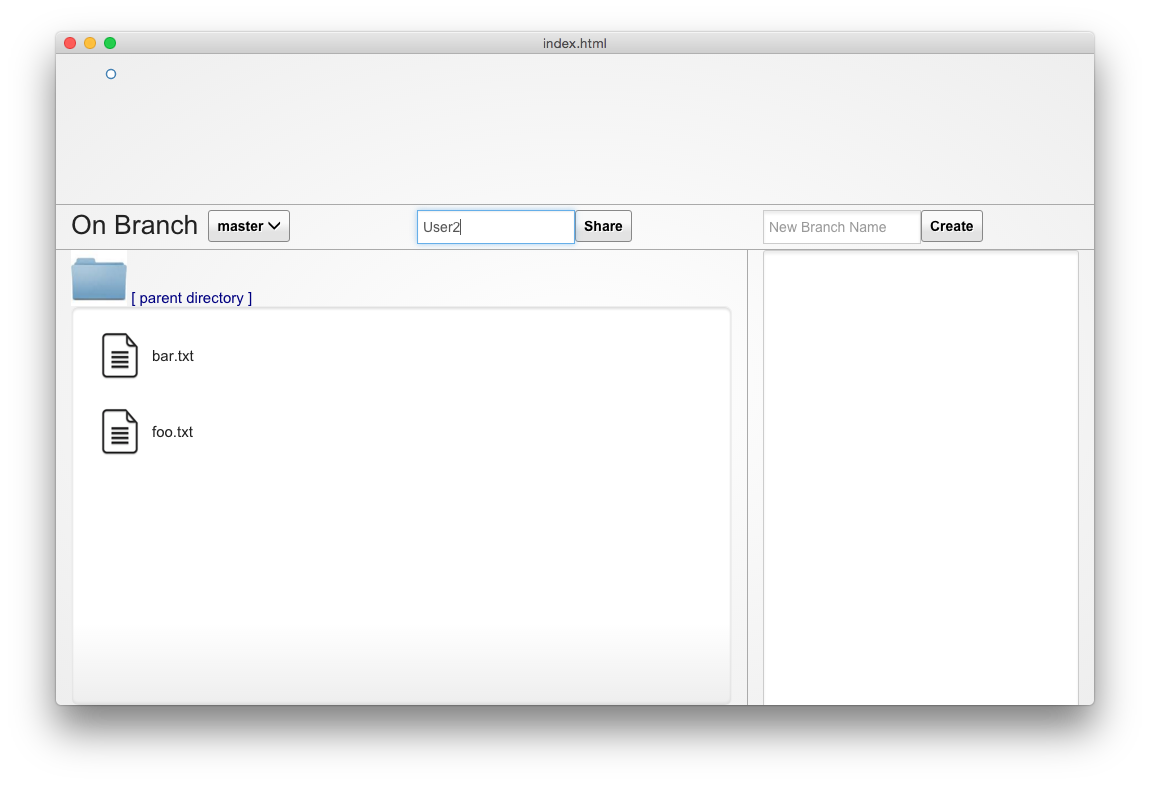
\includegraphics[width=0.82\textwidth]{SharingBranch1}
\caption{Sharing the ``master'' branch with user ``User2''.}
\label{arm:fig1}
\end{center}
\end{figure}

Figure 2-5 illustrates an example of two users working on a shared branch. When two snapshots are created at the same time, one will reach the upstream first. When this happens, that snapshot is confirmed and cannot be changed. When the second snapshot reaches the upstream, it will be rejected. Any snapshots that caused the rejection will be returned with the rejection to be inserted into the user's snapshot graph. The snapshot is then sent again and, if it is successfully added to the upstream, it will be sent to all collaborators on that branch.

\begin{figure}
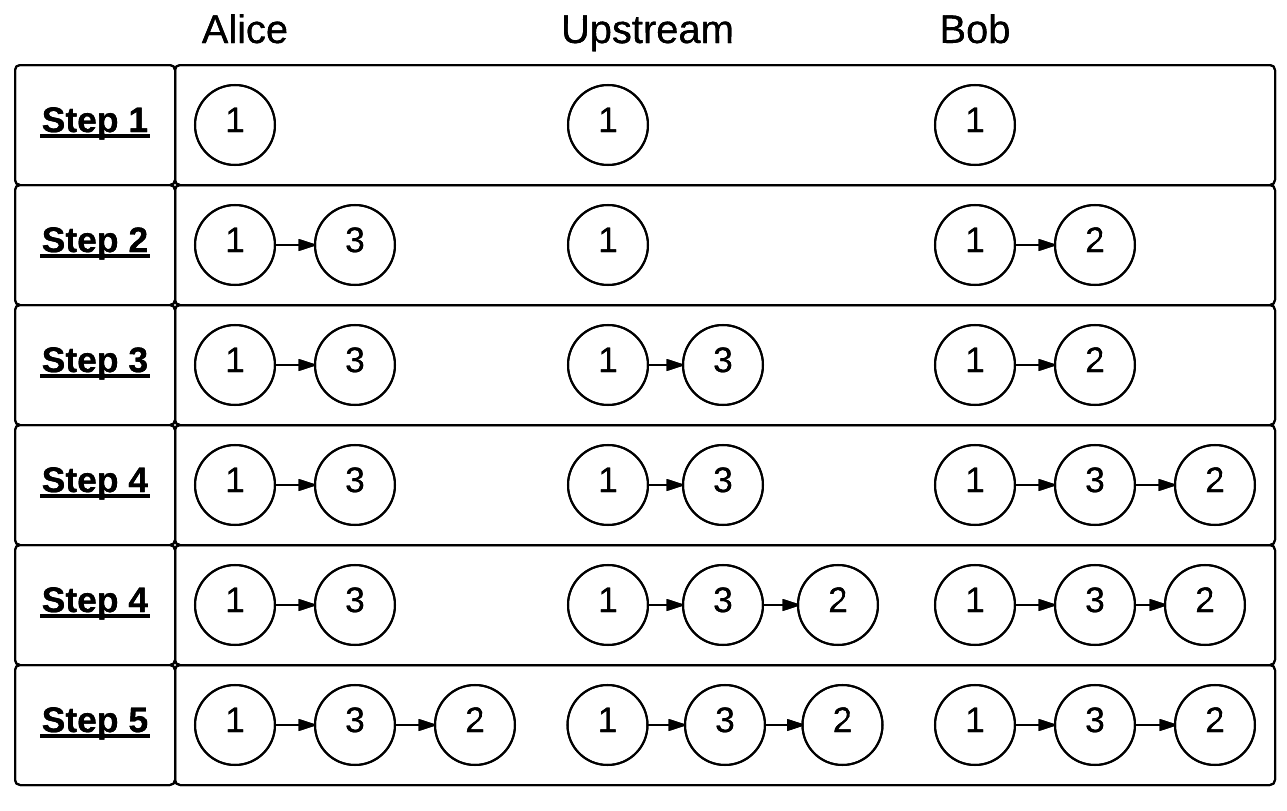
\includegraphics[max width= \linewidth]{Collaborating}
\caption{Conflicts being resolved on a shared branch.}
\label{arm:fig1}
\end{figure}

\subsubsection{Merging Branches}

Merging two branches compares the snapshot graphs in those two branches. If two snapshot graphs correspond to the same file, a merge is performed using three way merge and their common ancestor. This will result in a merge snapshot with as many parents as there are snapshots being merged. If there is a merge conflict, then the resulting snapshot will be a conflict snapshot. Like in Git, a conflict snapshot's content will show where the conflict needs to be resolved. Unlike in Git, this conflict snapshot is already saved in the local repository and any connected upstream repository; no conflict resolution is needed to continue working. By simply fixing the conflict and saving, a new snapshot is created that reflects the fix. Merging two branches will keep all of the group and tag data from both branches.

Figure 2-6 shows an overview of branch merging in Snapstore. Once snapshot graphs are identified as corresponding to the same file, their head snapshots are merged into a new snapshot, whose parents are the old head snapshots. In the figure, the head snapshots of ``foo.txt'', $3$ and $62$, are merged into a new merge snapshot, $4$. The snapshot graph of any file that does not have a counterpart in the other branch, like ``readme.txt'', will be copied over to the merged branch. If there is a file where a fast forward is needed instead of a merge, like ``bar.txt'', the snapshots will be copied and the head will move forward, but there will be no merge. 

\begin{figure}
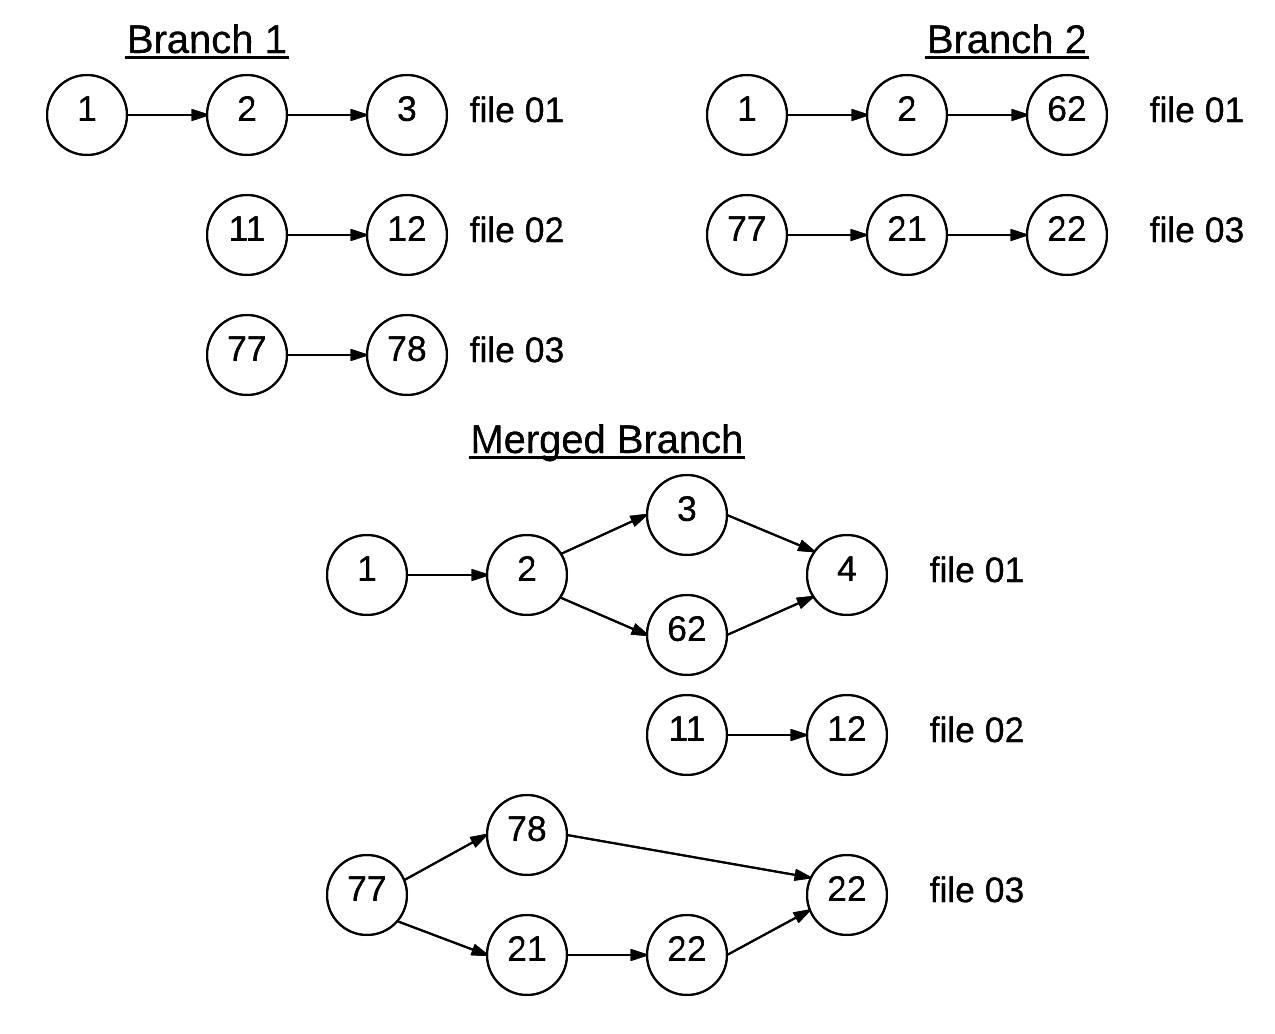
\includegraphics[max width= \linewidth]{Merging}
\caption{Merging two branches.}
\label{arm:fig1}
\end{figure}

\subsubsection{Using Branches to Support Complex Workflows}

Snapstore uses branches to allow users to partition their projects; they can then distribute these partitions to other users. This helps manage projects, and it can produce powerful workflows. Snapstore can achieve a workflow similar to that used by the Linux project and its system of trusted lieutenants who vet incoming contributions before passing them on to the project owner \cite{linux}.

Imagine that a website is being developed called ``Iweb''. The team creating this website has a project manager, a back-end developer, and a front-end developer. There is a master branch, ``Iweb-master'', that the project manager has access to. To partition this project, the project manager makes two clones of this branch, ``Iweb-front'' and ``Iweb-back''. ``Iweb-front'' contains all of the front-end code files, and ``Iweb-back'' contains all of the back-end code files. She shares ``Iweb-back'' with the back-end developer, and she shares ``Iweb-front'' with both the front and back-end developer because the back-end developer needs access to some of the front-end files.

A graphical representation of these branches, along with who has access to them, is included in Figure 2-7.

\begin{figure}
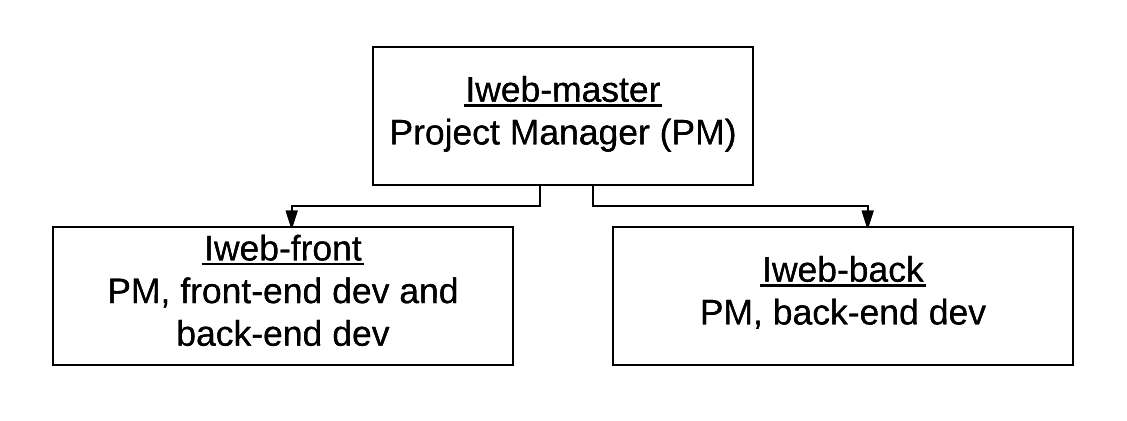
\includegraphics[max width= \linewidth]{caseStudy}
\caption{Iweb's branch arrangement.}
\label{arm:fig1}
\end{figure}

When edits are made by the developers, they are immediately seen by the project manager because they share the same branch. When the project manager decides that a certain branch, like ``Iweb-front'', is in a stable state, they can merge it with ``Iweb-master''.

This arrangement of branches accomplishes two things. First, it allows the project manager to vet edits to the cloned branches before merging them onto the master branch. Second, it allows some work to be hidden from some employees, achieving effective access control. The front-end developer does not have access to any of the files in ``Iweb-back''.

Note that this arrangement could be further expanded. The front-end developer, for example, could clone parts of the ``Iweb-front'' branch into more branches. Using this approach, Snapstore uses can achieve complex hierarchical workflows. 




